\chapter{Prototypische Umsetzung}     

Im folgenden Kapitel wird der Prototyp genauer betrachtet und die verschiedenen Aspekte seiner Entwicklung und Implementierung werden erläutert. Es werden dabei die verwendeten Technologien und die Art der Speicherung und Bereitstellung von Binärdaten beleuchtet. Um die Performance zu bewerten, werden Messungen auf generierte Testdaten durchgeführt.\\                               

\section{Überblick und Vorgehensweise}

Zunächst wird auf die eingesetzten Technologien eingegangen, die bei der Entwicklung des Prototyps verwendet werden. Dies umfasst das Framework Spring Boot, Programmiersprachen und andere Tools wie Terraform, die zur Umsetzung des Prototyps genutzt werden. Ein besonderes Augenmerk wird auf die Speicherung der Binärdaten gelegt. Hier werden verschiedene Ansätze betrachtet, wie beispielsweise die Verwendung von AWS SDK und Google Client Libraries. Des Weiteren wird die Bereitstellung der Binärdaten behandelt. Hier wird die Methode des Signed URLs betrachtet, um die Daten effizient an die Anwender zu übertragen. Um die Leistung des Prototyps zu bewerten, werden Testdaten mit zufälligem Inhalt generiert. Dies ermöglicht eine realistische Simulation der Tickets und Rechnungen in leoticket und erlaubt eine Bewertung der Performance der Cloud Provider. Die Messungen werden auf einem virtuellen Server durchgeführt, um eine präzisere Analyse zu gewährleisten.\\

Insgesamt bietet das Kapitel einen umfassenden Überblick über den Prototypen, seine Technologien, die Speicherung und Bereitstellung von Binärdaten sowie die Performance-Messungen. Es dient als Grundlage für weitere Untersuchungen und die Optimierung des Prototyps. 

\newpage

\section{Eingesetzte Technologien}

Für die Umsetzung des Prototyps werden die folgenden Technologien eingesetzt:

\begin{itemize}
	\item Spring Boot v3
	\item Terraform v1.4.4
	\item AWS SDK 2.0 Version
	\item Google Cloud Storage client library
	\item Java SDK 17 Temurin Version
	\item Maven v4.0.0
	\item AWS Toolkit
	\item aws cli
	\item gcloud cli
\end{itemize}

Für die Implementierung wurde als Entwicklungsumgebung Intellij Idea Ultimate verwendet. Intellij bietet das AWS Toolkit als Plugin an, das installiert werden kann. Als Framework wird die zum Zeitpunkt des erstellten Prototyps aktuellste Spring Boot 3 Version verwendet. Spring Boot stellt als Maven Dependency SDKs von beiden Cloud Anbietern zur Verfügung.

\begin{quote}
	Am 17. März 2021 wurde die neue Version des Spring Cloud AWS 2.3 veröffentlicht. Spring Cloud GCP und Spring Cloud AWS sind nicht mehr Teil des Spring Cloud Releases. Nicht Teil des Releases zu sein bedeutet auch, dass sie aus der Spring Cloud Organisation auf Github herausgenommen worden sind und dadurch neue Maven Package Namen haben. Das neue Package für Spring Cloud AWS heißt nun \glqq io.awspring.cloud\grqq, vgl. \cite{spring-cloud-announce}. 
\end{quote}

Die unten aufgeführten Maven Packages werden für AWS S3 und Cloud Storage verwendet:

\begin{code}
	<dependency>
        	<groupId>com.google.cloud</groupId>
        	<artifactId>spring-cloud-gcp-starter-storage</artifactId>
    </dependency> \end{code}

\begin{code}
	<dependency>
        	<groupId>io.awspring.cloud</groupId>
        	<artifactId>spring-cloud-aws-s3</artifactId>
        	<version>3.0.0</version>
    </dependency> \end{code}

Als Spring Cloud GCP Version wird die 4.2.0 verwendet. Beide Spring Cloud Packages werden von der Community auf Github verwaltet und aktualisiert. Für die Erstellung des Spring Boot Projekts wurde der Spring Initializier von Spring selbst verwendet unter \url{https://start.spring.io/}. Terraform wird für die Erstellung der Buckets in S3 und Cloud Storage verwendet. Die verwendete Terraform Version zum Zeitpunkt der Erstellung des Prototyp ist die 1.4.4. Zudem wird die Java SDK 17 Temurin Version verwendet. Für Maven wird die 4.0 Version verwendet.\\

Für die Authentifierung werden die aws cli und gloud cli verwendet. Diese werden über die offiziellen Dokumentationen installiert. Siehe \url{https://docs.aws.amazon.com/cli/latest/userguide/getting-started-install.html} für AWS CLI und  \url{https://cloud.google.com/sdk/docs/install?hl=de} für die gcloud CLI.  Das AWS Toolkit für die Authentifizierung mit AWS angewendet. Um sich mit Google Cloud zu verbinden wird eine Methode des ADC verwendet, welches im nächsten Abschnitt genauer erläutert wird.

\newpage

\section{Speicherung von Binärdaten}

Um Daten in S3 oder Cloud Storage speichern zu können, wurde der Prototyp so implementiert, dass der Nutzer sich zwischen S3 oder Cloud Storage entscheiden kann. Dies geschieht über die Klasse \textbf{CloudStorageServiceFactory}. Hier kann der Nutzer über die Environment Variable "cloud\_provider" den gewünschten Provider mit \glqq aws\grqq oder "google cloud" angeben. Dabei wird die Groß-, und Kleinschreibung nicht berücksichtigt. Die Environment Variablen können im System durch \glqq export <EnvironmentVariable>=<value>\grqq exportiert werden. Wenn eine IDE wie Intellij verwendet wird, kann dies unter den Run-Einstellungen als \glqq Environment Variables\grqq eingefügt werden. Nach der Eingabe des Cloud Providers wird das Programm die entsprechende Klasse aufrufen. Für AWS ist das die Klasse \textbf{AWSS3StorageService} und für Google Cloud die Klasse \textbf{GoogleCloudStorageService}. Beide Klassen implementieren von dem Interface \textbf{CloudStorageService}. Die \textbf{CloudStorageService} definiert zwei Methoden und eine davon ist für die Speicherung der Daten zuständig, siehe unteren Code:

\begin{code}
	void uploadObject(String bucketName, String key, String file, String encryptionKey) 
	throws IOException;
\end{code}

Dieser Methode wird der Bucket Name, der Name des Objekts, der Pfad des Objekts und der Encryption Key übergeben. Der Encryption Key kann dabei der Schlüssel sein, der in AWS KMS oder Google Cloud KMS generiert wurde. Die Implementierung dieser Methode ist für beide Cloud Provider ähnlich gestaltet.

\begin{figure}[h]
	\centering
	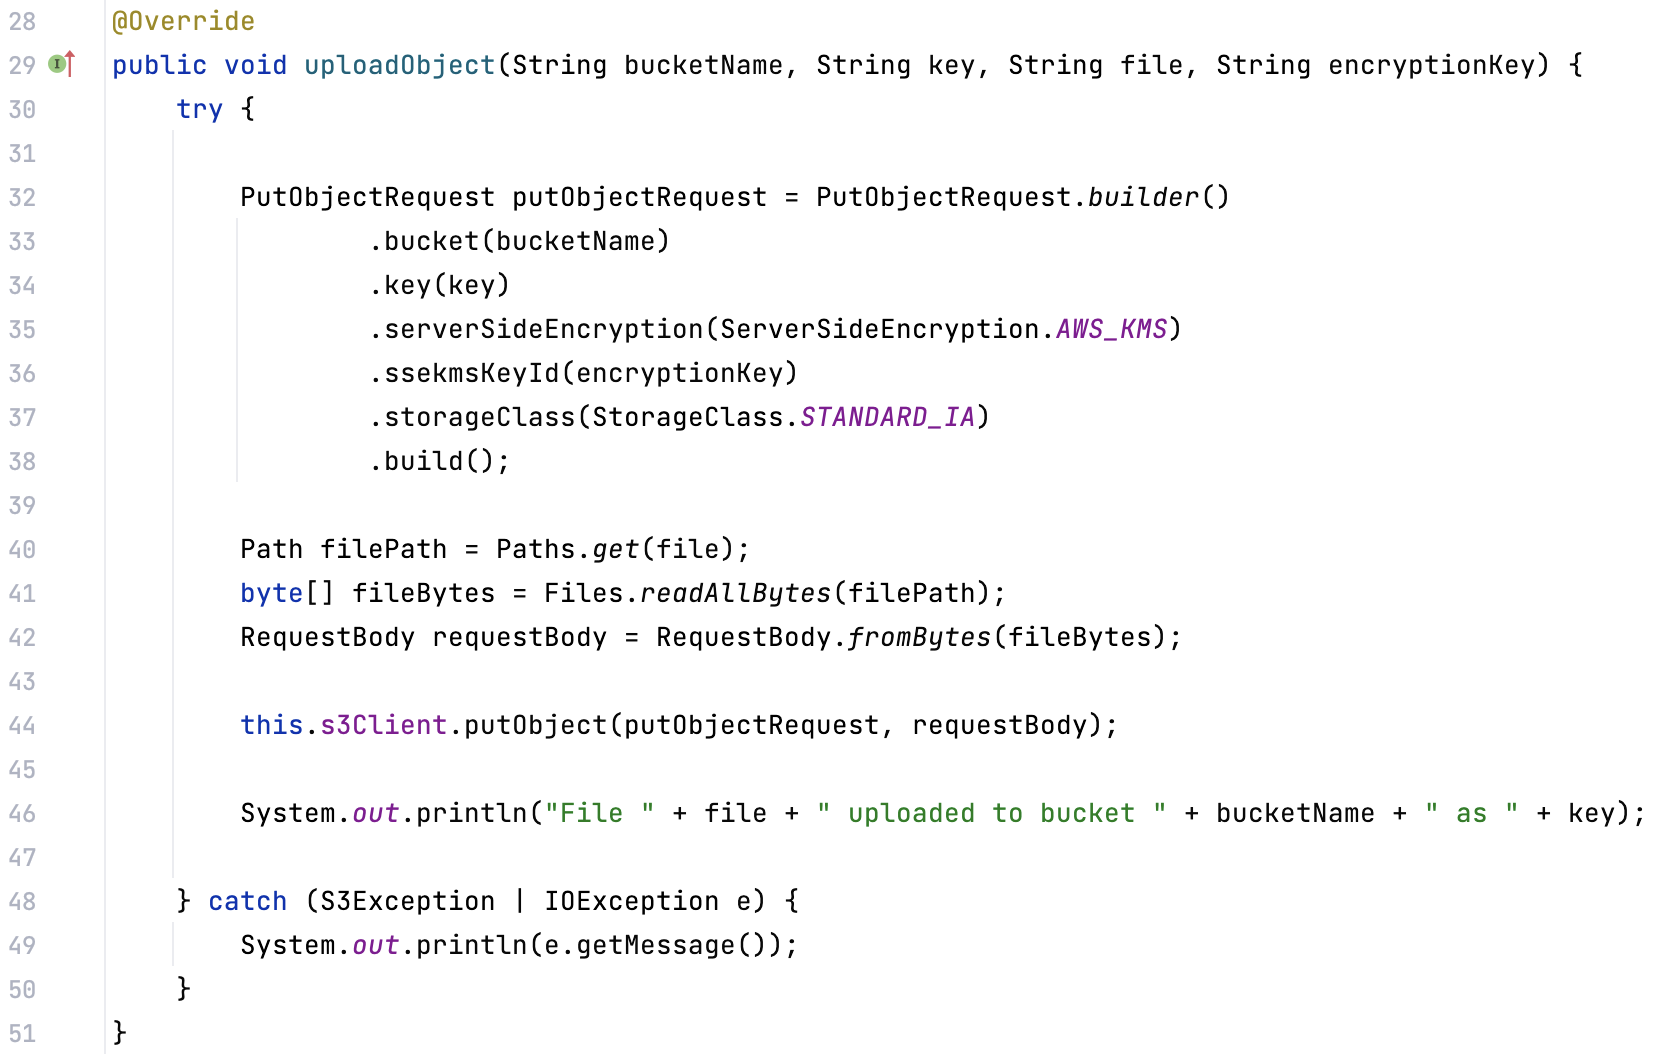
\includegraphics[width=15cm,keepaspectratio]{Pictures/UploadObjectAWS.png}
	\caption{Prototyp - Hochladen eines Objekts nach S3}
\end{figure}

\newpage

Der obere Code beschreibt den Speichervorgang eines Objekts nach AWS S3. Zuerst wird ein PUT Request Objekt erzeugt, indem die Parameter wie der Bucket Name, Objektname als Key und die Authentifizierungsmethoden angegeben werden. Es wird die AWS KMS Methode verwendet und den entsprechenden Schlüssel bereitgestellt. Zuletzt wird die Speicherklasse angegeben, indem das Objekt gespeichert wird. In diesem Beispiel wird die Standard - IA Klasse verwendet.\\

Anschließend wird der Pfad der angegeben Datei gelesen, als Bytes Array umgewandelt und dem RequestBody übergeben. Dieser RequestBody gemeinsam mit dem PutObjectRequest wird an den S3Client übergeben und mit der AWS .putObject() Methode nach S3 hochgeladen. AWS S3 verschlüsselt das Objekt mit dem angegeben Encryption Key und ladet es nach S3 hoch.\\

Die folgenden Abbildung zeigt den Code Ausschnitt von der Klasse GoogleCloudStorageService. Ähnlich wie bei der Methode für AWS S3 wird auch hier ein Objekt nach Cloud Storage hochgeladen. 

\begin{figure}[h]
	\centering
	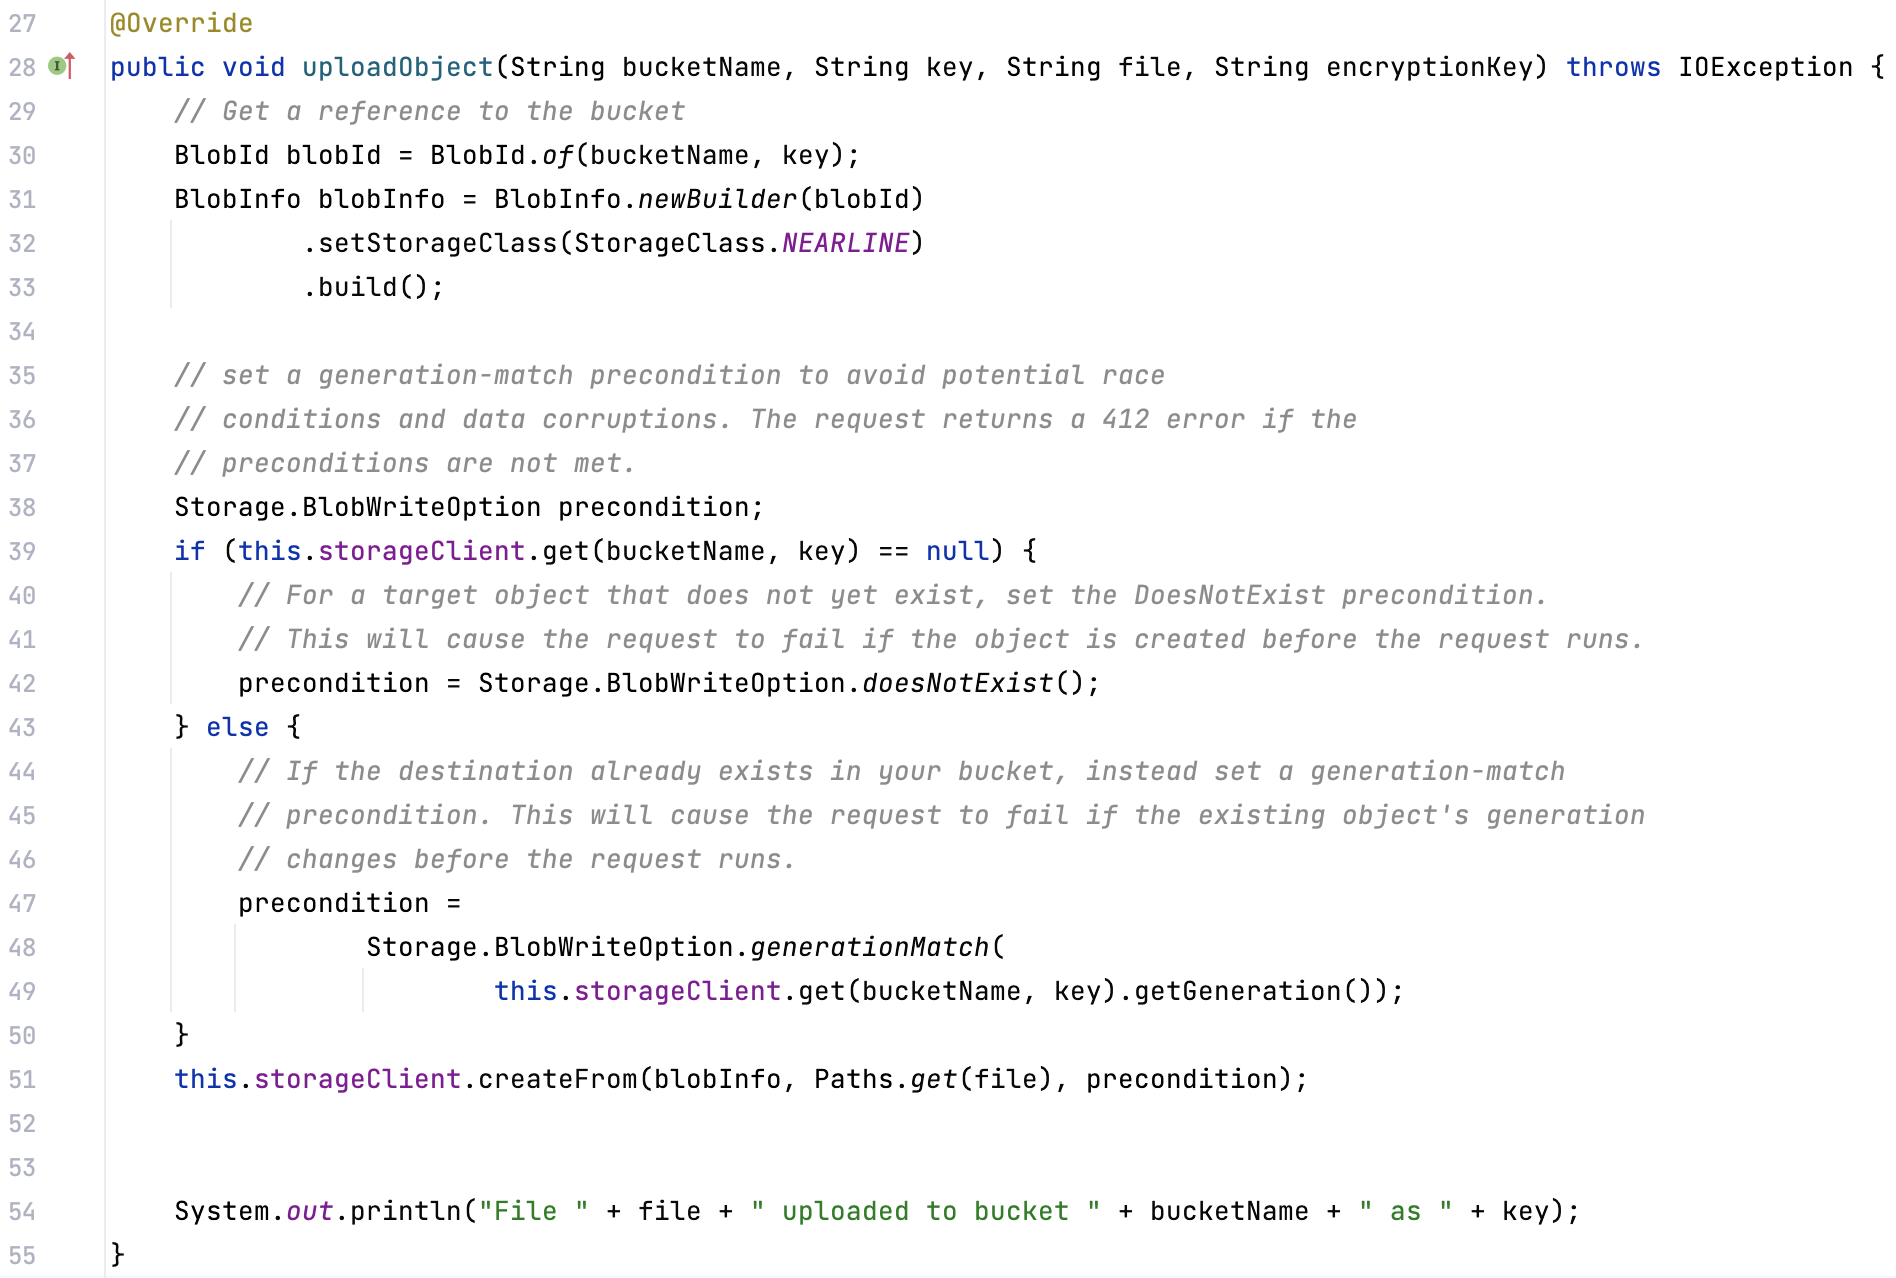
\includegraphics[width=15cm,keepaspectratio]{Pictures/UploadObjectGC.png}
	\caption{Prototyp - Hochladen des Objekt nach Cloud Storage}
\end{figure}

Dabei werden ähnliche Parameter der Methode wie in AWS S3 übergeben. Um ein Objekt in ein Bucket hochladen zu können, wird eine Referenz zum Bucket erstellt. Dies geschieht durch die BlobId, der den Bucket namen und den Namen des Objekts beinhaltet. Anschließend wird diese b†lobId dem BlobInfo Objekt übergeben und die Speicherklasse NEARLINE definiert. Nach dem überprüft worden ist, ob das Objekt bereits im Bucket existiert oder nicht, wird das Objekt in der Zeile 51 hochgeladen.\\

Um das Programm zum Laufen zu bringen, wird die Hauptklasse \textbf{HandsonAwsGcApplication} ausgeführt. Damit das Programm erfolgreich läuft, müssen die Environment Variablen im System exportiert werden. Alle Environment Variablen sind in der \glqq application.properties\grqq hinterlegt. Diese werden beim Start des Programms gelesen und angewendet. Außerdem müssen die AWS  und Google Cloud Credentials hinterlegt werden. Dies kann entweder über die AWS Toolkit Plugin gesteuert werden oder mit dem Befehl \glqq aws configure\grqq in der Kommandozeile. Für Google Cloud Credentials kann mit dem Befehl \glqq export GOOGLE\_APPLICATION\_CREDENTIALS=<service-account-json-file> der Service Account hinterlegt werden oder durch Ausführen des Befehls "gcloud auth application-default login\grqq in der Kommandozeile, was die Credentials lokal speichert und für ADC verwendet wird.


\section{Bereitstellung der Binärdaten}

\section{Messung der Performance auf Testdaten}

\subsection{Messungsergebnisse}

\section{Zusammenfassung der Implementierung}